\chapter{Heat Modeling of Integrated Devices}
\label{ch:heatmodeling}
\section{Heat Models using physical device models}
\subsection{Discrete Cosine Transform Approach}

\begin{center}
\begin{figure}[h]
\begin{center}
	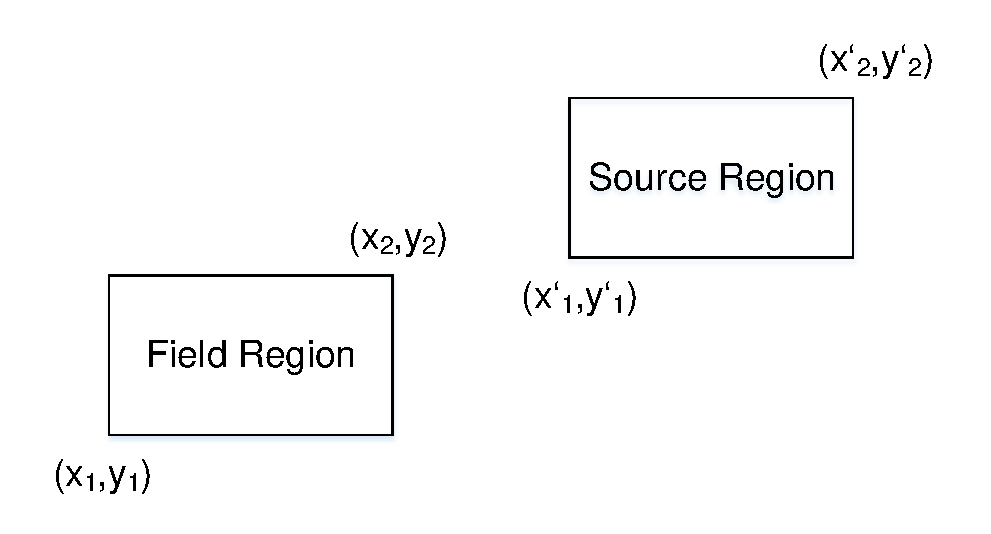
\includegraphics[width=0.8\textwidth]{__pics/regions}
	\caption{The temperature in the field region is derived from the power in the source region cf. \cite{Sapatnekar2005}}
	\label{pic:regions}	
\end{center}
\end{figure} 
\end{center}

\begin{equation}
\label{eq:hde}
\rho c_p \frac{\partial T(x,y,z,t)}{\partial t} =
\nabla \cdot [k(x,y,z,T) \nabla T(x,y,z,t)] +g(x,y,z,t)
\end{equation}

\begin{center}
	\begin{figure}[h]
		\begin{center}
			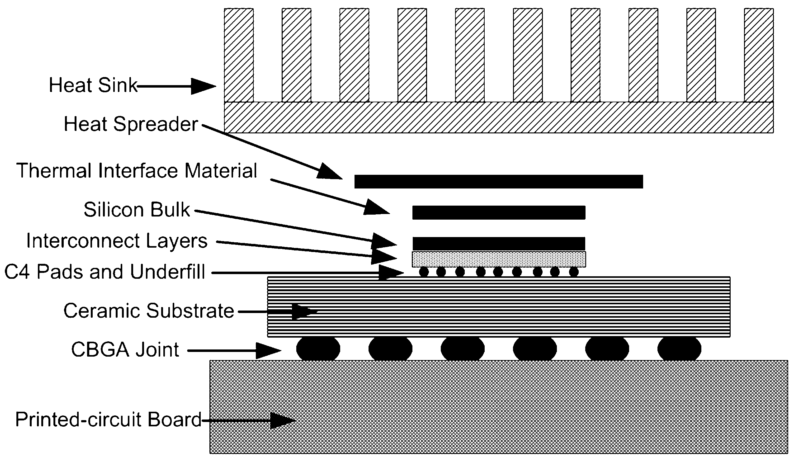
\includegraphics[width=0.8\textwidth]{__pics/packaging}
			\caption{Stacked layers in a typical \ac{CBGA} package \cite{Huang2006}}
			\label{pic:packaging}	
		\end{center}
	\end{figure} 
\end{center}

\subsection{HotSpot}
\cite{Huang2006}

\subsubsection{RC-\,Networks}
\label{ch:rcn}
\begin{center}
	\begin{figure}[h]
		\begin{center}
			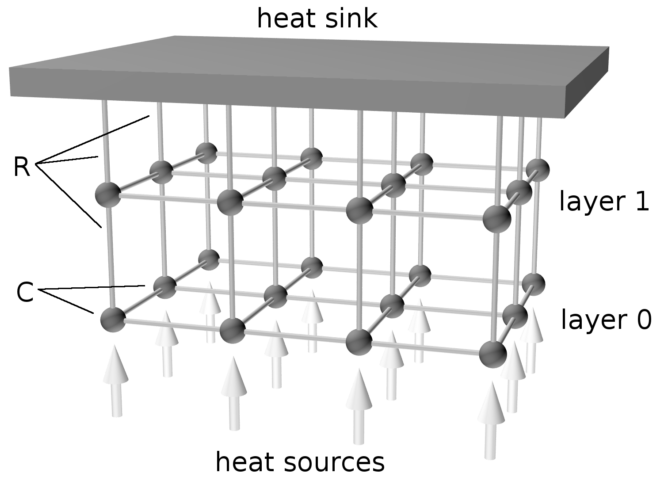
\includegraphics[width=0.7\textwidth]{__pics/rcn}
			\caption{RC-Network with two layers \cite{Happe}}
			\label{pic:rcn2}	
		\end{center}
	\end{figure} 
\end{center}


\section{Extension to On-Line Evolution of Heat Models}
\label{ch:ext}
\begin{itemize}
	\item RCN
	\item heat up
	\item cool down
	\item measure temperature
	\item learn parameters
	\item evaluate
\end{itemize}

\section{Temperature Measurement Methods}

\subsection{Built-In Temperature Sensor}
\label{sec:diode}
The most common way to measure temperatures on a \ac{VLSI} chip is to implement a temperature sensor in \ac{CMOS}. As stated in \cite{Bakker1996} the most effective way to achieve this goal is by using vertical bipolar transistors. This approach exploits the fact that the base-emitter voltage $V_{be}$ of a bipolar transistor decreases approximately by $2\,mV\symbol{23}^{\circ}C$ and hence almost linearly with the temperature. 
Furthermore, the difference between two measured base-emitter voltages $\delta V_{be}$ is almost linearly proportional to the absolute temperature $T_{abs}$ (ptat) and can be expressed as depicted in Equation~\ref{eq:PTAT}.

\begin{equation}
\label{eq:PTAT}
V_{ptat}(T_{abs}) = \frac{kT}{q}\cdot ln(p)
\end{equation}

The parameters for Equation~\ref{eq:PTAT} are the following:

\begin{itemize}
	\item Boltzman's constant, $k = 1.38 \times 10^{-23}$
	\item Temperature in Kelvin, $T [\symbol{23}^{\circ}\,K]$
	\item Charge on an electron in coulomb, $q = 1.6 \times 10^{-19}\,C$
	\item Emission current density ratio $p$
\end{itemize}

This temperature sensor achieves an accuracy of $\pm1\symbol{23}^{\circ}C$, by calibrating $V_{be}$ at room temperature \cite{Bakker1996}.

Also in modern \acp{FPGA} there is a trend of providing a pre-calibrated thermal diode, which are also provided at \ac{CMOS} level. These devices can for example be found at the Virtex-5 \ac{FPGA} by Xilinx, where the proportionality between the voltage and die temperature is as well exploited. Xilinx specifies this correlation with Equation~\ref{eq:XIL_PTAT} \cite{Xilinx2011a}.

\begin{equation}
\label{eq:XIL_PTAT}
V_{ptat}(T_{abs}) = 10 \cdot \frac{kT_{abs}}{q}\cdot ln(10)
\end{equation}

Note that the emission current density ratio is here set to $p = 10$. Hence, the temperature coefficient of $V_{ptat}$ is $-2\,mV/\symbol{23}^{\circ}C$.

Since the thermal diode is pre-calibrated, the temperature can be derived as depicted in Equation~\ref{eq:tempcalc}. To allow the further calculation it is mandatory to convert $V_{ptat}$, given as analog signal, into a digital number. The thermal diode on a Virtex-5 \ac{FPGA} digitizes $V_{abs}$ with the help of the built-in \ac{ADC} and produces the 10\,bit output \ac{ADC} code $V_ADC$. The resulting maximum-measurement error of this on-chip temperature sensor is specified with $\symbol{23}^{\circ}C$ \cite{Xilinx2011a}.

\begin{equation}
\label{eq:tempcalc}
	T[\symbol{23}^{\circ}C] = \frac{V_{ADC}\times 503.957}{1024} - 273.15
\end{equation}

\subsection{Infrared Cameras}
\label{sec:IRC}
Besides the above-named on-chip solutions of measuring the internal temperature, there is also the possibility to use \ac{IR} cameras. 

For instance, \cite{Ebi} measured a spatial thermal gradient of 2\symbol{23}$^{\circ}C$ over 10\,mm on a Xilinx Virtex II \ac{FPGA} using an \ac{IR} camera.
Furthermore \cite{Agne2013} used \ac{IR} cameras to illustrate temperature gradients of $15\symbol{23}^{\circ}C$, as depicted in Figure~\ref{pic:heater_infrared}. The four \ac{IR} camera pictures were taken in three second intervals. In each interval, temperature was generated in one of the chip's four corners. Inside the heated are the temperatures rose up to $95\symbol{23}^{\circ}C$ (depicted as black area), whereas the rest of the chip featured a temperature of $80\symbol{23}^{\circ}C$.

Using an \ac{IR} camera has the advantage of a high resolution. As stated in \cite{Nowroz2011}, \ac{IR} cameras can achieve a spatial resolution of up to $30\mu m$ with a $0.5\times$ microscopy kit. Furthermore, if the camera is set up properly, i.\,e. a direct view on the silicon and knowledge of the emission values, this approach provides accurate temperature information.
However, shortcomings of th \ac{IR} camera approach are that one always needs direct view on the chip's silicon layer \cite{Lopez-Buedo2004}. I.e. no heat sink, package or other material, where the emission values cannot be determined.
Besides the high price for these devices, \ac{IR} cameras cannot be employed in actual working conditions, because of their size \cite{Nowroz2011}.


\begin{figure}[h]
		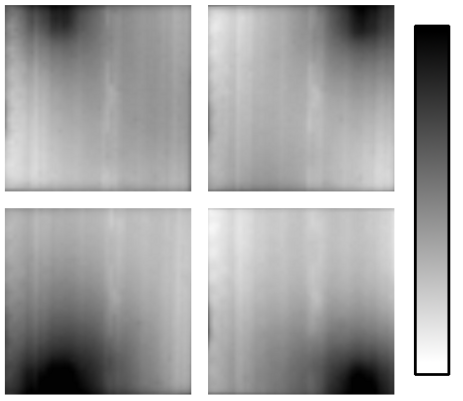
\includegraphics[width=\textwidth]{__pics/infra_heater}
		\caption{Four \ac{IR} images of the \ac{FPGA} with temperatures from 80\symbol{23}$^{\circ}C$ (white) to 95\symbol{23}$^{\circ}C$ (black) cf. \cite{Agne2013}}
		\label{pic:heater_infrared}	
	\end{figure} 

\subsection{Ring Oscillators}

Nowadays, a widely spread technique to measure the internal on-chip temperatures of \ac{FPGA}-based systems are based on \acp{RO}. These devices are composed of an odd number of inverters, which are connected in a chain. The endmost inverter's output is fed back to the first inverter. Figure~\ref{pic:simple_ro} depicts such a basic \ac{RO}. This leads to a device without a stable condition, causing each inverter's output to oscillate, i.\,e. the output $Q$ toggles between $0$ and $1$ and maximum speed with frequency $f_{osc}$. A longer inverter chain leads to a lower frequency and in addition to less power consumption \cite{Velusamy2005}.
It is because of the fact that the \ac{RO}'s frequency $f_{osc}$ is inversely proportinal to the on-chip temperature \cite{Lopez-Buedo2002}, that \acp{RO} can be used to measure the temperature on any location on the \ac{FPGA}. The output frequency $f_{osc}$ is dependant on the curcuit's delay. Furthermore, it is also known that \acp{RO} can be used in order to measure delay, leakage and dynamic power \cite{Zick2010, Zick2012}. 

\begin{figure}[h]
		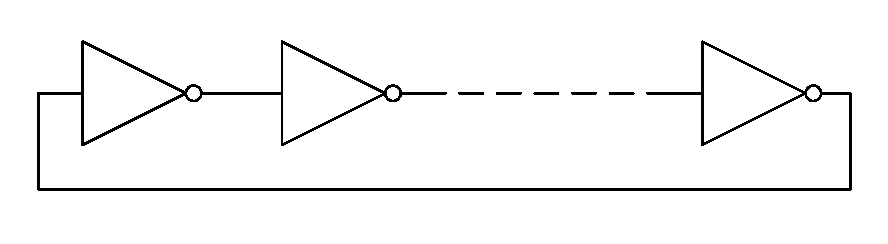
\includegraphics[width=\textwidth]{__pics/RO.pdf}
		\caption{A basic Ring Oscillator, consisting of an odd number of inverters}
		\label{pic:simple_ro}	
	\end{figure} 

\subsubsection{Methodology}

Measuring the internal on-chip temperature necessarily requires knowledge about the frequency $f_{osc}$ of the \ac{RO}. In order to estimate the frequency, several approaches \cite{Sayed2011, Lopez-Buedo2002, Velusamy2005, Happe} make use of \acp{RO} combined with a capture counter. The counter, as depicted in Figure~\ref{pic:Temp_Sensor}, is clocked with a system \ac{CLK} and by the oscillating output $Q$ of the \ac{RO}. $Q'$ toggles at the speed of $Q$ and is sampled by \ac{CLK}. Put simply, the capture counter samples the number $S$ of oscillations at the signal $Q'$ with the frequency $clk$. Afterwards the sampled number of oscillations can be derived to $f_{osc}$. 

\begin{figure}[h]
		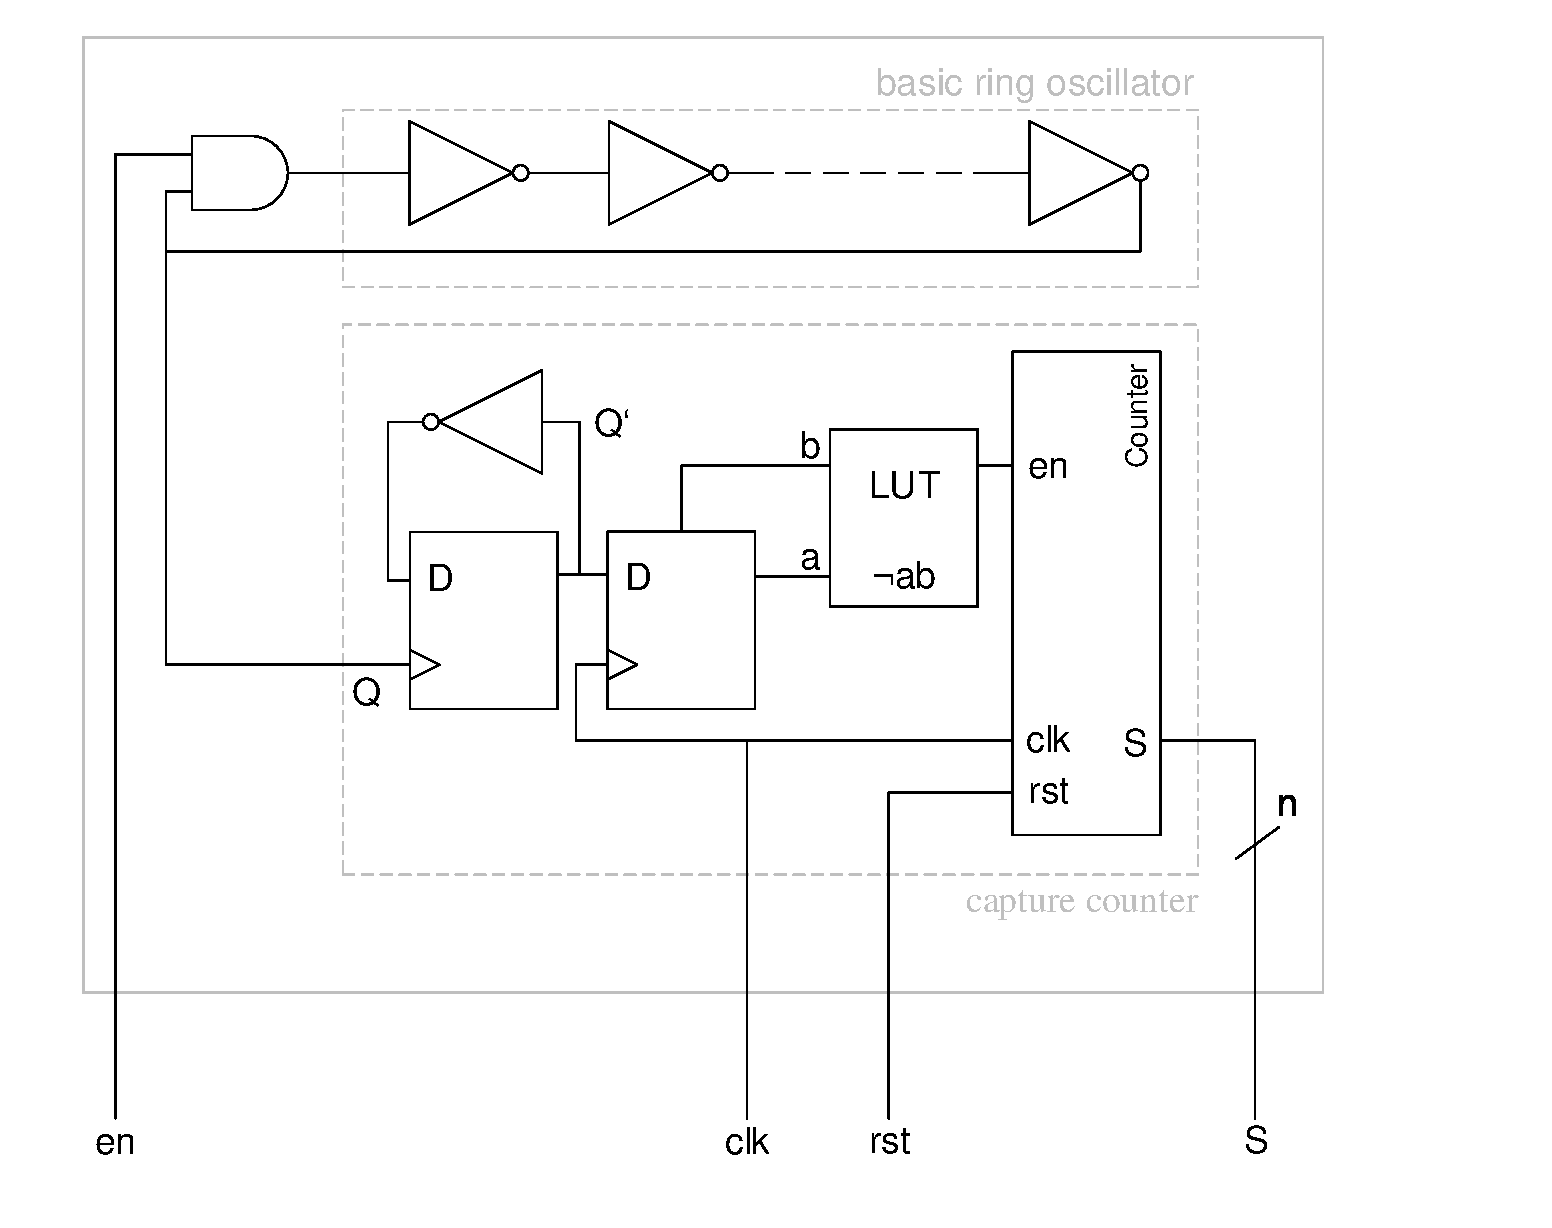
\includegraphics[width=1.15\textwidth]{__pics/Temp_Sensor.pdf}
		\caption{Simplified schematic of a temperature sensor with capture counter cf. \cite{Ruthing2012}}
		\label{pic:Temp_Sensor}	
	\end{figure} 
	
However, there are also differences in implementing the \ac{RO}-based temperature sensor. These variable parameters are: number of inverters, system routing, length of measurement period $t_m$ and the possible use of latches between the inverters. 
The use of latches was proposed in order to minimize the impact of routing \cite{Zick2012}. For \acp{FPGA} designs, it is advisable to use latches instead of the additional wiring between the inverters. 

The benefits of designing on an \ac{FPGA} are the reconfigurability. This possible due to the \acp{CLB} of which the \ac{FPGA} is composed. The \ac{CLB} however comprises slices, which contain \acp{LUT} and \acp{FF}. 
Hence, by using \acp{LUT} for the \ac{RO}'s inverters, the \acp{FF} can be used as latches without significant additional wiring.

In contrast to previous approaches, which used seven \cite{Happe} or eleven inverters \cite{Lopez-Buedo2002, Velusamy2005} and no latches, a high-performance \ac{RO}-based temperature sensor comprises 23 inverters and 24 latches \cite{Ruthing2012}. The quality of the \ac{RO} is derived by the sensor's resolution and noise/deviation.
In addition to the utilization, the optimal measurement period $t_m$ should not exceed the maximum length of $2^{16}$ clock cycles, which is $655\,\mu s$, when the counter samples with 100\,MHz. For longer measurement periods, there is a risk of self-heating, since \acp{RO} may lead to considerable temperature gradients \cite{Agne2013}.

As previously pointed out, the optimal measurement with the proposed temperature sensor includes the following steps \cite{Ruthing2012}:

\begin{itemize}
	\item Enable \ac{RO} with 23 inverters and 24 latches
  \item Wait $2^{12}$ -- $2^{16}$ clock cycles so that the \ac{RO} can gain a constant frequency
  \item Sample $Q'$ for $t_m$ clock cycles
  \item Disable the \ac{RO}
  \item Read out the counter value $S$.
\end{itemize}

\subsubsection{Calibration Methods}

Given the sensor count $S$ of \ac{RO}-based temperature sensors, it is not possible to predict a function that maps $S$ to a temperature $T$. Instead, the sensors need to be calibrated with an pre-calibrated device, such as the built-in thermal diode, a temperature-controlled oven or an \ac{IR} camera. 
While the device is heated up and cooled down afterwards, $S$ is counted and the temperature is read in regular time intervals. For each sensor placed on the chip the linear mapping function is then determined by partial regression \cite{Lopez-Buedo2002, Ruthing2012}. 

The following approaches request for a temporal temperature gradients equally distributed on the chip. Section~\ref{sec:tempgen} will give an overview of most common and useful methods for heating up the sensors, e.g. the \ac{RO}-based temperature sensors.

As proposed in \cite{Lopez-Buedo2002} the sensors were calibrated by an iron-constantan (Fe-CuNi) thermocouple which is placed in the centre of the package exactly measure the on-chip temperature $T$.

Section~\ref{sec:IRC} already illustrated that \ac{IR} cameras are able to exactly measure the on-chip temperature $T$ \cite{Nowroz2011}, provided that the camera is pointing directly on the silicon and the emission value is known. Additionally of course, they can be used for calibrating the \ac{RO}-based temperature sensors with high accuracy. 

Also, temperature-controlled ovens might be used for calibrating the sensors. Because by setting and thereby knowing the surround temperature of the die, $T$ and $S$ can also be captured.

Another way to calibrate the sensors is to make use of the built-in thermal diode, which was presented in Section~\ref{sec:diode}. While heating up the chip, the sensor data $S$ and the diode temperature $T_{diode}$ are captured. Note that this diode has $\pm 4�C$ inaccuracy and is assumed to be in the centre of the \ac{FPGA} \cite{Agne2013}.

\subsection{Discussion on Accuracy and Calibration}

The above-named approaches all fit well in the application of measuring temperatures and - if the devices are pre-calibrated - calibration of other sensors. However, each has benefits and shortcomings, which are listed in Table~\ref{tbl:proconmeasurement}. The thermal diode, which is built-in in many nowadays \acp{FPGA} benefits from being easily accessible via the system monitor. Using this temperature sensor requires no additional implementation or calibration. On the other hand the specified accuracy of $\pm 4\symbol{23}^{\circ}C$ may be to much. Furthermore, this accuracy can possibly not be met in real life. As depicted in \cite{Sayed2011}, the diode has measured incorrect temperatures compared to an external thermometer. On a Xilinx Virtex-5 \ac{FPGA} the difference between both devices amounts to $20.3\symbol{23}^{\circ}C$. Until now, it has not been resolved why this differences occurs.
Another disadvantage of using the thermal diode is that it is not clear where on the \ac{FPGA} it is placed, though it is assumed to be in the centre of the \ac{FPGA} \cite{Agne2013}. Hence the diode is not able to detect on-chip hot spots or the specific temperature of a certain instantiated circuit on the \ac{FPGA}.

A much more accurate approach is the use of \ac{IR} cameras. It is able to measure the on-chip temperatures with a high resolution, i.\,e. everywhere on the \ac{FPGA}. This again leads to the possibility of detecting hot spots.
On the other hand, \ac{IR} cameras are not only very expensive but very bulky, which hinders the in-field application. Beyond that, you need to have direct vision onto the silicon, which requires unpacking of the die.

The most effective way to measure temperatures on reconfigurable devices is using \ac{RO}-based temperature sensors. It has nearly the advantages compared to \ac{IR} cameras, and is beyond that easy to implement in reconfigurable computing devices. However, these sensor network needs to be calibrated. As this work aims to reconfigurable devices, i.\,e. \acp{FPGA}, the only handy and imaginable approach is the thermal diode, which could be a disadvantage in occurrence of incorrect measurements.


\begin{center}
\begin{table}

\begin{center}
\begin{tabular}{|p{3.16cm}|p{3.16cm}|p{3.16cm}|}
	
	\hline  \textbf{Measurement Technique} & \textbf{Pro} &  \textbf{Contra} \label{tab:proconmeasurement}\\ 
	\hline \hline  \textbf{Thermal diode} & Built-in and pre-calibrated & Inaccuracy and no hot spot detection \\ 
	\hline  \textbf{\ac{IR} camera} & Very accurate, high resolution and hot spot detection & Very expensive, no usage in field, requires view on silicon and knowledge about emission values \\ 
	\hline  \textbf{\ac{RO}-based sensor} & High resolution and hot spot detection & Calibration \\ 
	\hline
\end{tabular} 
\caption{Advantages and Disadvantages of several temperature measurement techniques}
\label{tbl:proconmeasurement}
\end{center}
\end{table}
	
\end{center}

\section{Temperature Generation Methods}
\label{sec:tempgen}

As said earlier most sensors, e.\,g. \ac{RO}-based, have to be calibrated before use. In order to do so accurately, the \ac{IC} needs to be heated up to learn about the sensor output in combination with a pre-calibrated sensor temperature output.
But besides that, it might be interesting to heat up devices for the sake of evaluating the functionality. This may include fault tolerance like timing or soft and hard errors under occurrence of heat, especially for scientific use.

Several approaches are using a temperature-controlled oven in order to heat up the chip \cite{Velusamy2005, Lopez-Buedo2002}. This way, the \ac{IC} is heated up and simultaneously the \acp{RO} are calibrated. In the first instance, these approaches use heat generation for calibration. But as a matter of principle, temperature controlled ovens can be used to heat up \acp{IC} uniformly distributed on the die.
Practically, on the other hand, it might also be interesting to create local hot spots and generate spatial gradients on the chip in order to learn about the chip's thermal properties. Temperature controlled ovens do not support this kind of researching, not least because of the needed bulky external device.
A much handier way to calibrate sensors might be the laser trimming \cite{Bakker1996}, which is out of place in the field of reconfigurable computing, for instance for designing on \acp{FPGA}.

A better way, which also perfectly matches the advantages of reconfigurable computing is the use of dedicated heat generating circuits, specified in Verilog or \ac{VHDL}, following the approach of self-heating. By instantiating the low level components of a \ac{FPGA}, several approaches achieved temperature increases and local hot spots on the die. These components are mostly placed in the \ac{FPGA}'s \ac{CLB} and comprise

\begin{figure}[h]
	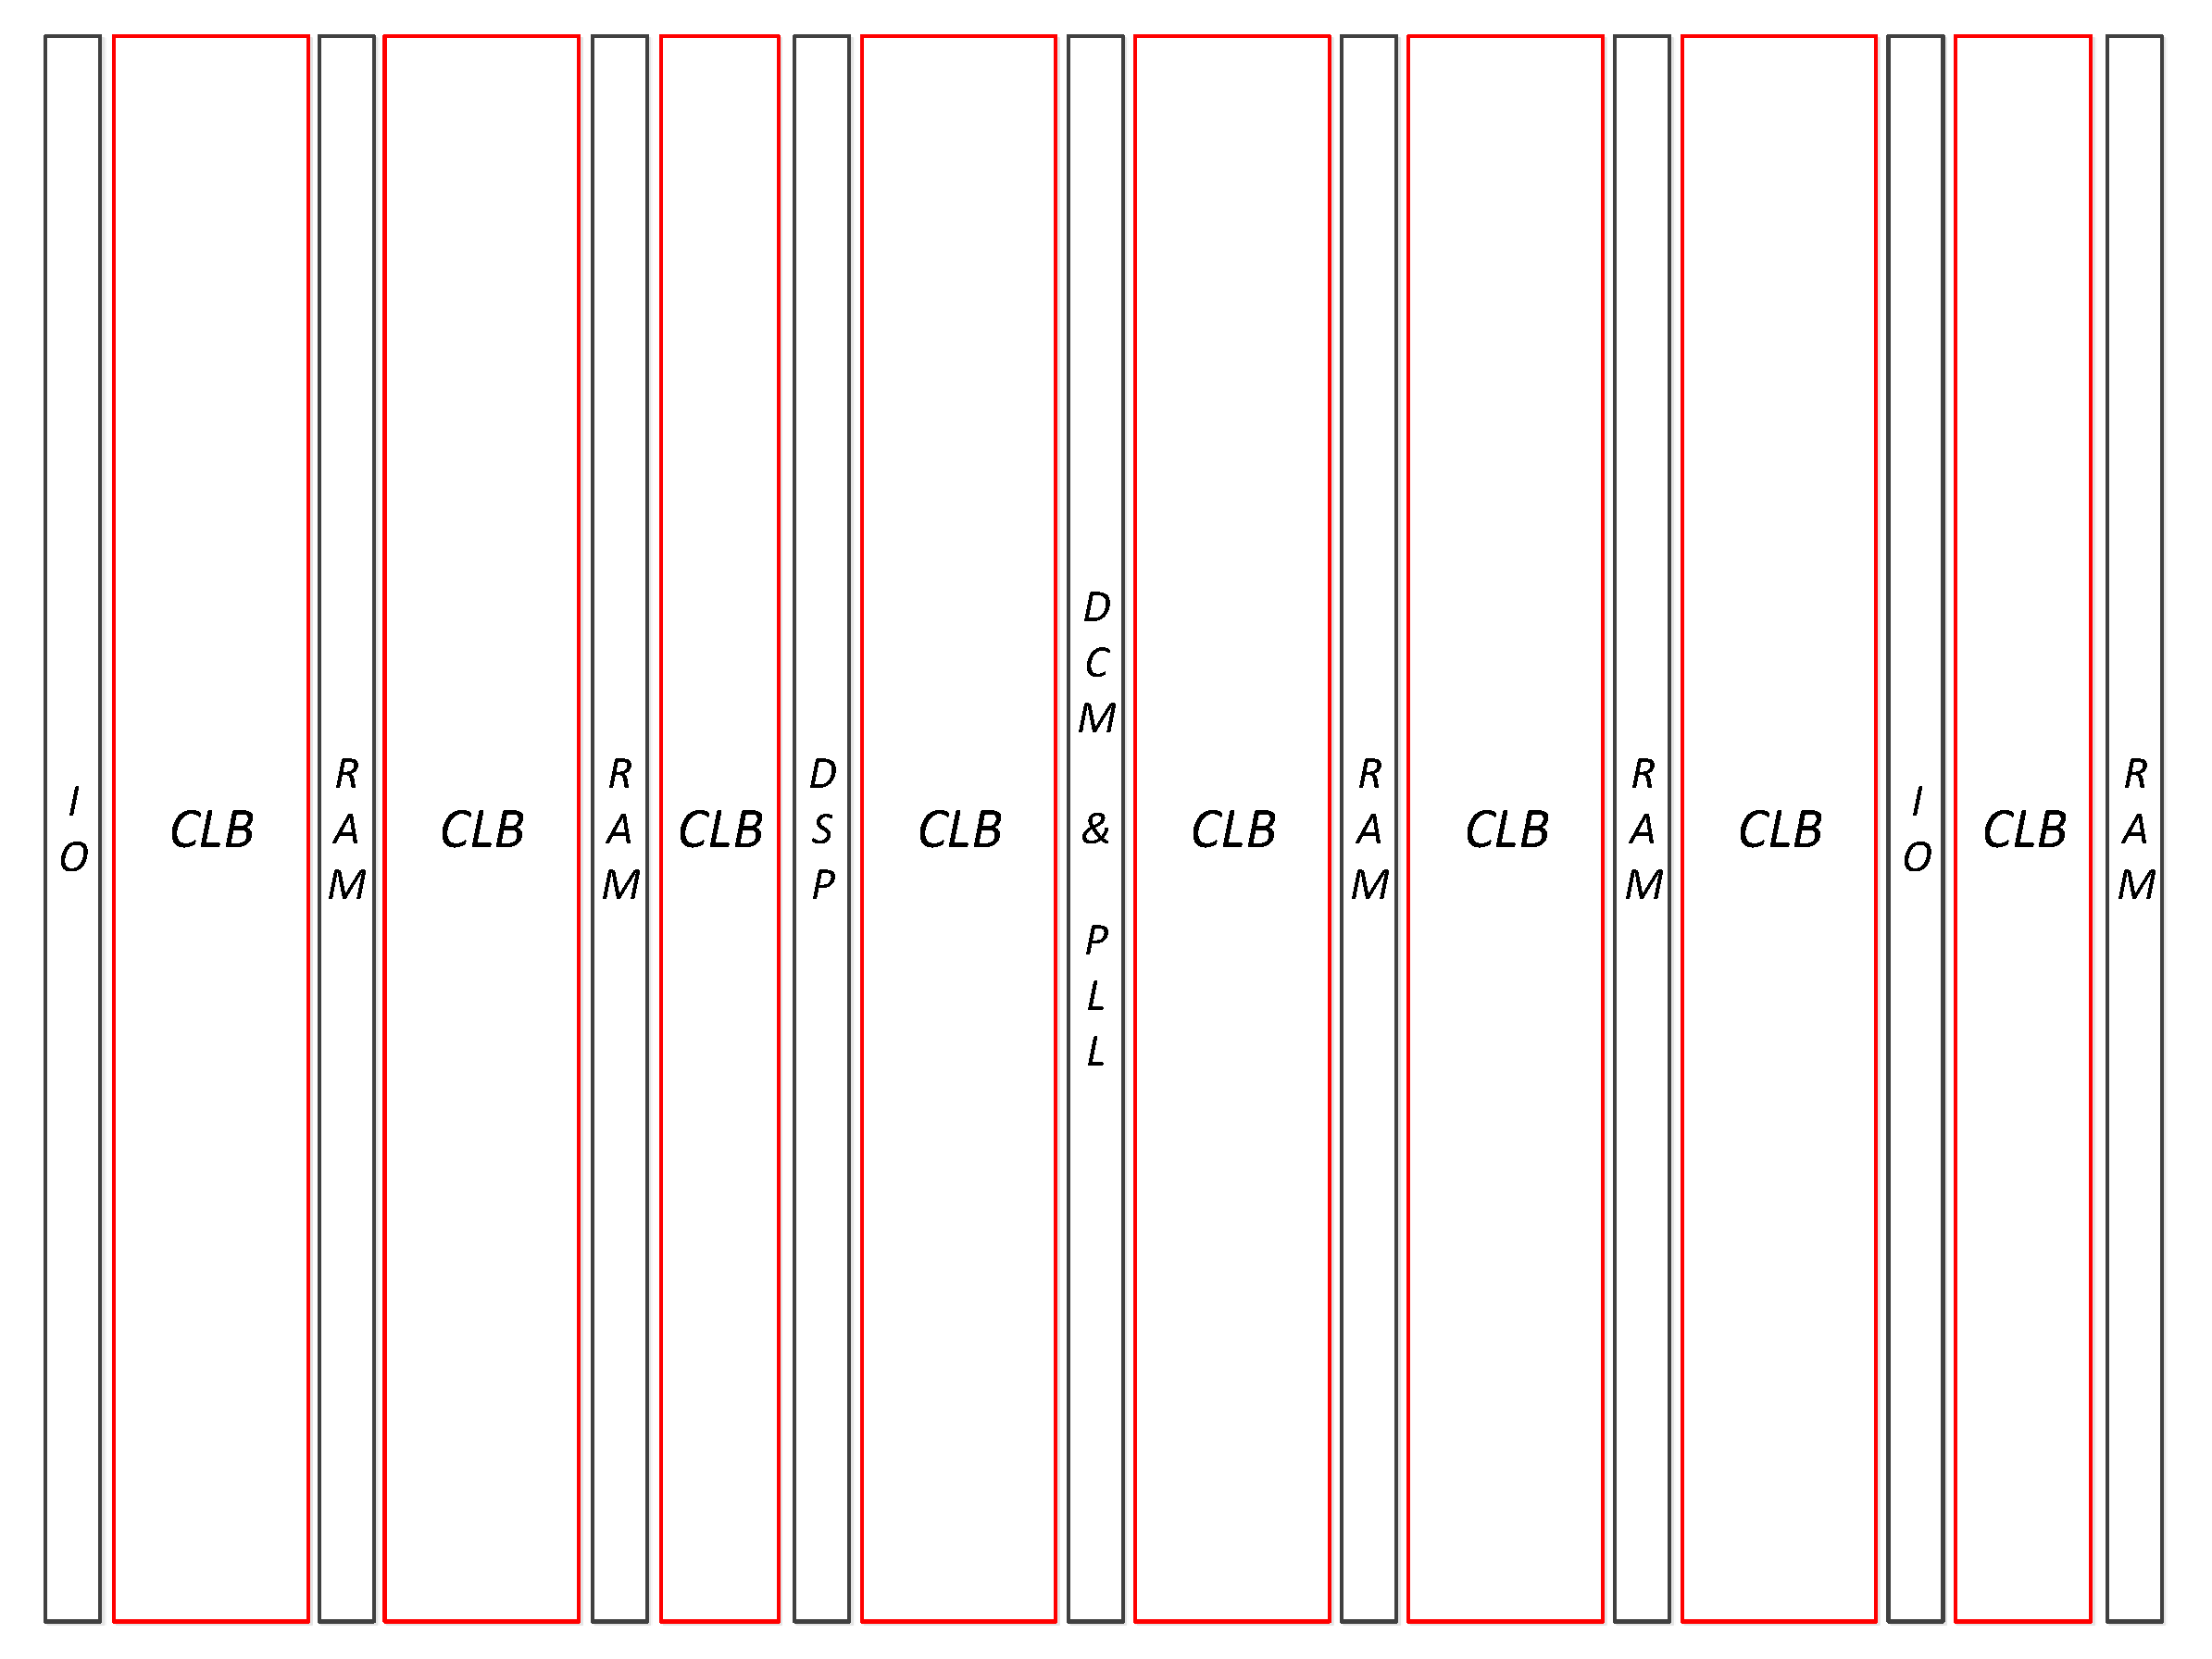
\includegraphics[width=\textwidth]{__pics/v5.pdf}
	\caption{A simplified overview of a Virtex-5 \ac{FPGA}}
	\label{pic:v5}	
\end{figure}

\begin{itemize}
	\item \acp{LUT}\\
			Arranged in the \ac{CLB}'s slices. \acp{LUT} can implement any \textit{n}-input logic function. The highest amount of input signals \textit{n} is nowadays 6. Logical functions with a higher amount in input signals can be achieved by combining several \acp{LUT}
	\item \acp{FF}\\
			Also stored in slices next to \acp{LUT}. \acp{FF} can be initialized with a start value.
	\item \acp{DSP}\\
			\ac{DSP} blocks are compact and high-speed circuits and fulfil the special purpose of huge arithmetical and logical operations. Usually there is a special area between some \acp{CLB}
	\item \acp{BRAM}\\
	       Also arranged between several \ac{CLB}. \acp{BRAM} can for instance be used as \ac{FIFO}, single or dual port \ac{RAM}.
\end{itemize}

Figure~\ref{pic:v5} depicts the arrangement of these components on Virtex-5 \ac{FPGA}. Additionally \ac{IO} blocks, \ac{DCM} and \ac{PLL} are added.

It is easy to see that the most effective way to generate temperature increases and especially local hot spots or spatial temperature gradients is to use the \acp{CLB}, i.\,e. \acp{LUT} and \acp{FF}. The designer is thereby almost not restricted to an area that can be heated. 
As illustrated in \cite{Sayed2011} the used \ac{FPGA} increased its temperature up to 37$\symbol{23}^{\circ}C$ by utilizing $80\%$ of the \acp{CLB}. More precisely, the \acp{LUT} and \acp{FF} were arranged in a pipeline as depicted in Figure~\ref{pic:lutffpipe}, clocked at $100\,MHz$. The output of each \ac{LUT} was wired with the input of another \ac{FF}, whose output was on the contrary was wired to another \ac{LUT} and so on.

\begin{figure}[h]
	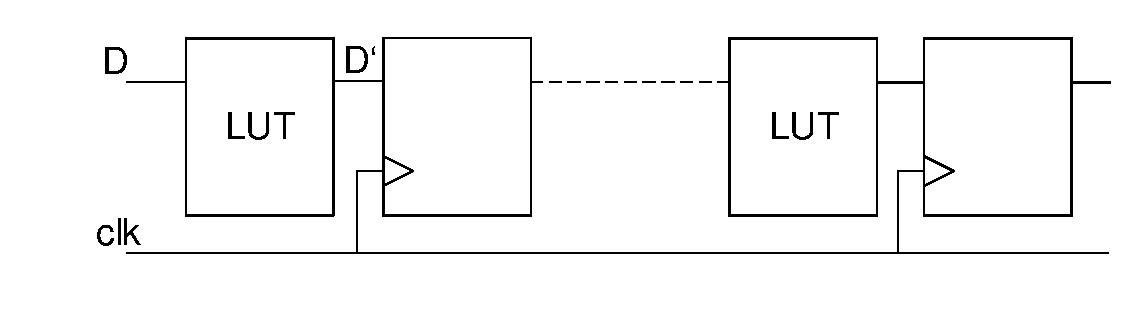
\includegraphics[width=\textwidth]{__pics/LUTFFpipe.pdf}
	\caption{ Pipeline consisting of \acp{LUT} and \acp{FF}}
	\label{pic:lutffpipe}	
\end{figure}

\begin{figure}[h]
	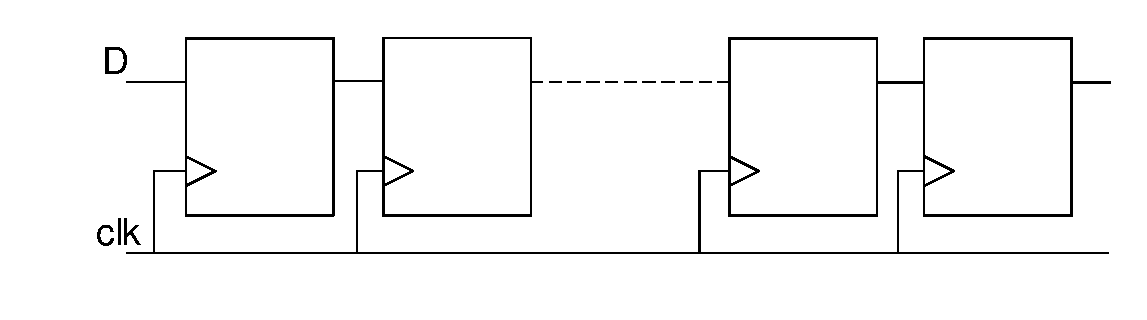
\includegraphics[width=\textwidth]{__pics/FFpipe.pdf}
	\caption{Pipeline consisting of \acp{FF} }
	\label{pic:ffpipe}	
\end{figure}

Local hotspots were for instance created by using a \ac{FF} pipeline as illustrated in Figure~\ref{pic:ffpipe}. As \cite{Happe} depicted, it is possible to create a spatial gradient of $6.5\symbol{23}^{\circ}C$ by utilizing 10.000 \acp{FF} on the \ac{FPGA}, which were clocked at $100\%$.

As a systematic study of possible heat generating circuits yielded, there are even more temperature increases and spatial gradients possible \cite{Agne2013}. A average overall temperature rise of $81.2\symbol{23}^{\circ}C$ was achieved by implementing 1.000 single-level oscillators on the \ac{FPGA}. As Figure~\ref{pic:lutosc} depicts, this oscillators were realized with \acp{LUT}, which fed back the outputs to the input \textit{I0}. The logical function that was stored in this \ac{LUT} is a simple \ac{XOR}, which function as an inverter, when the enabling signal is activated. This slim and effective heat generating circuit also achieved a spatial temperature gradient of up to $10\symbol{23}^{\circ}C$.

\begin{center}
\begin{figure}[h]
\begin{center}
	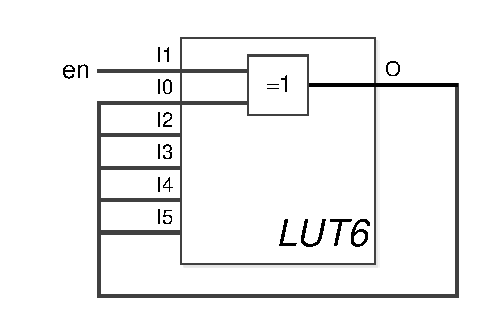
\includegraphics[width=0.70\textwidth]{__pics/lutoscillator.pdf}
	\caption{\ac{FPGA}-Implementation of a 1-level \ac{RO}}
	\label{pic:lutosc}	
\end{center}
\end{figure} 	
\end{center}